\chapter{Introducere}
\label{chapter:intro}

Viața celor mai multora dintre noi este strâns legată de tehnologie. Avem peste tot în jur și folosim sisteme informatice; cu ajutorul acestora ne informăm, comunicăm, ducem la bun sfârșit activități profesionale și personale.

Un sistem informatic este compus din sisteme de calcul, infrastructură și date. Sistemele de calcul sunt echipamentele cu putere de procesare pe care le folosim direct sau indirect (servere, laptopuri, telefoane mobile); infrastructura înseamnă rețeaua, sistemele de stocare, interfețele de acces.

Acest elemente formează lumea informației digitale, sau lumea IT \& C (Information Technology and Communication). Este lumea care definește revoluția tehnologică a ultimelor decenii, lumea care definește funcționarea majorității domeniilor: economie, politică, educație, societate.

Oricare dintre noi este un utilizator de tehnologie informatică. În general, facem acest lucru prin intermediul dispozitivelor și sistemelor de calcul personale: sistem desktop, laptop, smartphone, smart TV, smartwatch. Un sistem de calcul (\textit{computer system}) sau un dispozitiv de calcul este o componentă fizică ce poate prelua, prelucra și reda informație. De exemplu, un smart TV primește comenzi prin telecomandă, preia conținut video de pe Netflix, îl prelucrează și apoi îl redă utilizatorului pe ecran. Un laptop preia acțiuni de la utilizator ce pot rezulta în pornirea unei aplicații de tip browser web și accesarea platformei Facebook pe care utilizatorul să o urmărească.

Un utilizator cu profil tehnic, care dorește o utilizare mai eficientă sau mai sigură a sistemului de calcul, sau care dorește personalizarea acestuia, va urmări să înțeleagă dedesubturile funcționării acestuia.

Această carte este destinată înțelegerii funcționării unui sistem de calcul din perspectiva unui utilizator cu profil tehnic, accentul fiind pus pe sistemul de operare, o componentă software esențială a sistemului de calcul. Majoritatea noțiunilor prezentate sunt comune tuturor sistemelor de calcul și sistemelor de operare; însă ne vom concentra pe sisteme de calcul de tipul desktop / laptop și pe sistemul de operare Linux.

\section{Sisteme de calcul}
\label{sec:intro:computer-systems}

Așa cum am precizat mai sus, un sistem de calcul este un echipament care preia informații, le prelucrează și le livrează mai departe. Îl mai numim și calculator. În engleză termenul este de \textit{computer/computing system} sau \textit{computer}. Definiția este destul de relaxată pentru a include un număr mare de dispozitive: de la servere cu mii de procesoare și putere de prelucrare imensă până la dispozitive portabile precum smartwatch-uri. În general, pe parcursul acestei cărți vom folosi interschimbabil noțiuni precum sistem de calcul, dispozitiv de calcul, dispozitiv, platformă de calcul, echipament.

Pe parcursul unei zile putem folosi mai multe sisteme de calcul din posesia noastră sau a altora:

\begin{itemize}
  \item avem pe birou un sistem desktop în care dezvoltăm aplicații
  \item avem o consolă pentru jocuri
  \item avem un smart TV pe care urmărim cele mai recente episoade din serialul preferat
  \item avem un ruter Wi-Fi cu care avem acces la Internet
  \item avem un laptop pe care navigăm pe Internet, lucrăm cu documente, testăm aplicații
  \item avem un dispozitiv mobil inteligent (\textit{smartphone}) cu care ascultăm muzică, discutăm cu cei apropiați, accesăm platforme de socializare
  \item avem un asistent activat vocal (\textit{smart speaker}, precum Google Home sau Amazon Alexa) care poate fi comandat pentru a furniza informații, pentru a reda o melodie, pentru a consulta calendarul
  \item avem un smartwatch pe care avem informații despre starea de sănătate, avem remindere și avem acces la calendar și informații despre vreme
  \item avem un computer de bord în mașină cu care ascultăm muzică din telefon, cu care accesăm hărți pentru navigație
  \item accesul pe platforme de hărți sau de socializare sau de conținut video sau audio înseamnă folosirea Internet-ului și a unor sisteme de calcul de tip server aflate la distanță într-un data center întreținut de companii precum Google, Amazon sau Facebook
\end{itemize}

Aceste sisteme de calcul sunt folosite de majoritatea utilizatorilor, indiferent de pregătirea lor tehnic. Un utilizator cu profil tehnic tehnic, care lucrează sau este pasionat de lumea calculatoarelor (IT\&C) va folosi și alte sisteme de calcul. Iar folosirea unui sistem de calcul duce, prin Internet, la folosirea altor sisteme de calcul.

Un sistem de calcul este compus din hardware (componente fizice) și software (programe sau aplicații). Cele două componente funcționează împreună; hardware-ul oferă puterea de calcul în vreme ce software-ul oferă o interfață flexibilă și prietenoasă utilizatorului, ca în \labelindexref{Figura}{fig:intro:computing-system}.

\begin{figure}[htbp]
  \centering
  \def\svgwidth{\columnwidth}
  \includesvg[width=0.3\textwidth]{chapters/00-intro/img/hw-sw-user.svg}
  \caption{Sistemul de calcul și utilizatorul}
  \label{fig:intro:computing-system}
\end{figure}

Cea mai importantă caracteristică a software-ului este flexibilitatea. Se poate configura o aplicație existentă pentru a funcționa diferit sau se pot instala noi aplicații. Nu este nevoie de o schimbare de echipament cum ar fi în cazul hardware-ului.

În general, spunem că un sistem de calcul este compus din hardware și software-ul necesar utilizării de bază. Alte componente software ce vor fi adăugate ulterior de utilizator nu fac parte din sistemul de calcul. Din nou, definiția este relaxată, nu există o graniță clară între ce componente software sunt necesare utilizării de bază și ce componente software sunt necesare unei utilizări specifice.

Componenta esențială a software-ului unui sistem de calcul, și subiectul principal al acestei cărți, este sistemul de operare. Sistemul de operare gestionează resursele fizice/hardware ale sistemului de calcul și facilitează folosirea acestora de aplicații. \labelindexref{Figura}{fig:intro:computing-software} prezintă organizarea unui sistem de calcul, cu aplicațiile rulând peste sistemul de operare.

\begin{figure}[htbp]
  \centering
  \def\svgwidth{\columnwidth}
  \includesvg[width=0.6\textwidth]{chapters/00-intro/img/computing-software.svg}
  \caption{Componentele software într-un sistem de calcul}
  \label{fig:intro:computing-software}
\end{figure}

O categorie aparte de aplicații sunt aplicațiile de sistem (\textit{system programs}, \textit{system software}). Aceste componente software oferă suport suplimentar celorlalte aplicații; o aplicație de sistem importantă este shellul. Shellul oferă utilizatorului interfața cu care acesta să poată porni și interacționa cu alte aplicații. Acesta poate fi grafic sau în linie de comandă. Mai multe despre shell și interfața cu utilizatorul vom discuta în \labelindexref{Capitolul}{chapter:ui}.

În continuare vom detalia sistemul de operare.

\section{Sistemul de operare}
\label{sec:intro:os}

Un sistem de operare este un set de programe folosite pentru a gestiona resursele hardware ale sistemului. Sistemul de operare ascunde complexitatea hardware-ului de aplicații. Un dezvoltator de aplicații nu este preocupat de diferențele hardware între diferitele platforme, ci doar de interfața pe care o oferă sistemul de operare.

Spunem că sistemul de operare îndeplinește următoarele roluri:

\begin{itemize}
  \item abstractizare hardware: sistemul de operare oferă o interfață pentru aplicații; indiferent de specificul hardware, interfața va fi aceeași
  \item portabilitate: aceeași aplicație (de pildă browserul web Firefox sau editorul Vim) poate rula nemodificată pe același sistem de operare aflat pe configurații hardware diferite ale sistemului (cu procesoare sau discuri sau plăci de rețea diferite)
  \item mediere: sistemul de operare asigură accesul echitabil al mai multor aplicații la resursele hardware; dacă două aplicații folosesc simultan Internetul, sistemul de operare va transfera pe rând informațiile către/de la acestea folosind placa de rețea a sistemului, având în vedere să nu amestece fluxurile de transfer
  \item securitate/izolare: fiecare aplicație rulează izolat de celelalte; o aplicație nu va folosi neautorizat și nu va corupe, accidental sau cu intenție, resursele altei aplicații
\end{itemize}

Unele dispozitive nu au sistem de operare, acestea fiind în general, dispozitive cu rol specific (\textit{embedded systems}) care rulează o singură aplicație. Exemplu de astel de dispozitive sunt un proiector, un bec inteligent, un senzor de lumină sau de temperatură. Dispozitivele și sistemele de calcul au însă un sistem de operare, sau o componentă software alternativă.

Componenta centrală a sistemului de operare, cea care gestionează și abstractizează resursele hardware este \textbf{nucleul sistemului de operare}, numit și \textbf{kernel}. Nucleul sistemul de operare este o componentă critică, coruperea ducând la coruperea întregului sistem. Nucleul abstractizează resursele hardware oferind aplicațiilor o interfață numită interfața de apeluri de sistem (\textit{system call interface}), la fel ca în \labelindexref{Figura}{fig:intro:syscall-interface}. O aplicație care are nevoie de acces la resursele hardware sau o anumită funcționalitate implementată de sistemul de operare va invoca un apel de sistem prin interfața de apeluri de sistem.

\begin{figure}[htbp]
  \centering
  \def\svgwidth{\columnwidth}
  \includesvg[width=0.5\textwidth]{chapters/00-intro/img/syscall-interface.svg}
  \caption{Interfața de apeluri de sistem}
  \label{fig:intro:syscall-interface}
\end{figure}

Utilizatorul nu este preocupat de obicei de sistemul de operare și nu interacționează cu acesta. În afară de câteva informații de forma ,,pe laptop am Windows'' sau ,,am telefon cu Android'', utilizatorul nu are nevoie să afle mai multe. Lucrurile se schimbă pentru un utilizator cu profil tehnic; pentru acesta este interesant să înțeleagă sistemul de operare și particularitățile sale pentru a putea folosi mai eficient, mai sigur sau mai pe gustul său sistemul de calcul.

Din punctul de vedere al utilizării, putem considera următoarea clasificare a sistemelor de operare:

\begin{itemize}
  \item sisteme de operare generaliste, folosite pe sisteme server, desktop sau laptop: Microsoft Windows, Apple macOS, distribuții GNU/Linux, FreeBSD
  \item sisteme de operare pentru dispozitive mobile: Android, Apple iOS
  \item sisteme de operare specializate: pentru echipamente de rețea (Cisco iOS, Juniper Junos OS, DD-WRT), pentru smartwatch-uri (Apple watchOS, Wear OS), pentru smart TV (Tizen, webOS, Apple tvOS), pentru console de jocuri (Sony Orbis OS, Microsoft Xbox OS, Nintendo Horizon) etc.
\end{itemize}

Clasificarea este una evolutivă, nu strictă. Pot fi adăugate tipuri noi pe măsură ce anumite dispozitive apar. Dacă am fi făcut o clasificare similară în 2005, de exemplu, a doua categorie (sisteme de operare pentru dispozitive mobile) nu ar fi existat.

E de remarcat că sistemele de operare sunt legate între ele deși rulează pe sisteme de calcul radical diferite. De exemplu, GNU/Linux, Android, DD-WRT, Wear OS, Tizen, webOS au la bază kernelul Linux; adică sunt sisteme de operare derivate din același kernel. La fel este cazul produselor Apple (macOS, iOS, watchOS, tvOS): au la bază sistemul de operare Darwin. Pentru un utilizator tehnic, cunoașterea unui sistem de operare înseamnă că va avea o bază de cunoștințe pentru diferitele platforme pe care acesta rulează.

\subsection{Alegerea sistemului de operare}
\label{sec:intro:pick}

Alegerea unui anumit sistem de operare ține de mai mulți factori, important fiind ce urmărește utilizatorul și pe ce sistem de calcul va rula sistemul de operare. Cu toate acestea, pentru o bună parte din dispozitive, întrebarea apare rar sau deloc. De exemplu, pentru un cumpărator de smart TV sau de consolă de jocuri nu va conta sistemul de operare în alegerea produsului, va conta produsul în sine. Puțini utilizatori sunt preocupați de sistemul de operare care rulează pe ruterul lor wireless, e important să funcționeze corespunzător. În general, întrebări și alegeri au loc în cazul sistemelor de operare generaliste (server/desktop/laptop) și a dispozitivelor mobile inteligente (smartphone).

În cazul dispozitivelor mobile inteligente (smartphones), cele mai răspândite sisteme de operare sunt Apple iOS și Android. Alegerea între cele două ține de mai multe criterii. Internetul abundă de comparații între cele două. În plus, în vreme ce Apple controlează dispozitivele și sistemul de operare de pe iPhone, ecosistemul Android este mult mai vast. Cineva poate alege un anumit telefon cu Android ținând cont mai mult de diferențele hardware decât de cele software (mai reduse). Un sumar al avantajului fiecărei platforme este mai jos:

\begin{itemize}
  \item Android: Dispozitivele Android sunt mai diverse și, în general, mai ieftine. Un utilizator poate decide ce telefon să își achiziționeze dintr-o plajă largă de opțiuni. Aplicațiile Android se pot dezvolta pe orice platformă folosind, uzual, mediul Android Studio, în vreme ce aplicațiile iOS se dezvoltă doar pe macOS folosind mediul Xcode.
  \item iOS: Dispozitivele iPhone, care rulează iOS, sunt produse uniform de Apple și în general, dispun de o mai bună integrare a componentelor software/hardware. Ecosistemul Apple oferă avantaje: o integrare foarte bună cu alte componente și tehnologii Apple (macOS, tvOS, iCloud, iTunes), versiuni puține și stabile de sisteme de operare.
\end{itemize}

Sistemele de operare generaliste rulează pe sisteme de calcul puternice, care cuprind o unitate de calcul și periferice precum monitor, tastatură, mouse. Aceste sisteme pot fi servere, folosite pentru prelucrări de date în general de organizații, sau sisteme desktop sau laptop, folosite de utilizatori obișnuiți. Dintre sistemele de operare generaliste cele mai cunoscute și folosite sunt Microsoft Windows, Apple macOS și GNU/Linux.

La fel ca în cazul Android/iOS, pe Internet sunt numeroase articole comparative între cele trei sisteme de operare generaliste de mai sus, cu avantajele și dezavantajele fiecăruia. De avut în vedere că migrarea tot mai multor aplicații în zona web înseamnă că diferențele dintre sisteme de operare sunt din ce în ce mai reduse. Adesea un utilizator se va descurca la fel de bine și pe Windows și pe macOS și pe Linux pentru că va petrece o bună parte din timp folosind un browser web, care oferă o interfață relativ comună. Mai jos sumarizăm avantajele fiecăruia și cazurile frecvente de utilizare:

\begin{itemize}
  \item Microsoft Windows: Este cel mai răspândit sistem de operare pe sistemele desktop, multe sisteme desktop/laptop venind cu Microsoft Windows preinstalat. Are integrare cu produsele enterprise Microsoft, folosite în companii și organizații mari. Cele mai multe aplicații dezvoltate rulează pe Windows. Jocurile sunt dezvoltate în special să ruleze pe Windows.
  \item Apple macOS: Vine preinstalat pe dispozitive produse de Apple (MacMini, MacBook) și vine preconfigurat. Oferă un mediu de lucru mai aproape de Linux pentru dezvoltatorii tehnici. În general urmărește utilizabilitate, atât la nivel software și interfața cât și la nivel hardware: greutate laptop, aspect, tastatură, durată baterie.
  \item GNU/Linux: Este cel mai răspândit sistem de operare pe sistemele server, fiind fiabil și cu multe aplicații pentru dezvoltatori și administratori. Oferă o plajă diversă de distribuții, poate fi personalizat și configurat. Este un sistem open source, adică este accesibil codul sursă, un foarte bun mod de învățare și de participare în cadrul comunității de dezvoltatori.
\end{itemize}

Un utilizator va opta pentru folosirea unui sistem și în funcție de preferințe personale și de nevoie; de exemplu, poate nu este mulțumit cu un anumit sistem de operare, dar o anumită aplicație rulează numai pe acela; sau la locul de muncă i se cere să folosească un anumit sistem de operare.

Poate apărea situația în care un utilizator are nevoie să folosească 2 sisteme de operare, pentru nevoi sau preferințe diferite. În această situație are două opțiuni:

\begin{enumerate}
  \item dual-install/dual-boot: pe același sistem de calcul instalează două sisteme de operare diferite și pornește alternativ unul sau altul. Detalii tehnice prezentăm în \labelindexref{Capitolul}{chapter:boot}.
  \item mașină virtuală: instalează un sistem de operare într-o mașină virtuală și folosește acea mașină virtuală din sistemul de operare principal. Detalii tehnice prezentăm în \labelindexref{Capitolul}{chapter:vm}.
\end{enumerate}

În general, un sistem desktop sau laptop vine cu un sistem de operare preinstalat. Utilizatorul are posibilitatea instalării altui sistem de operare, a instalării dual-boot sau a instalării unei mașini virtuale. Imediat după instalare, utilizatorul va face configurațiile de bază: crearea unui cont de utilizator, configurarea datei, schemei de tastatură, personalizarea interfeței grafice. Apoi va folosi sistemul în scopul dorit, folosind aplicații deja existente sau instalând aplicații noi.

În această carte vom prezenta noțiuni conceptuale ce se aplică în general, pe toate tipurile de sisteme de calcul și sisteme de operare. Pentru aspecte demonstrative, vom folosi ca suport Linux pe desktop. Aceasta pentru că sistemul de operare și distribuțiile bazate pe Linux, fiind open source, oferă acces rapid și deschis la resursele interne ale sistemului. În Linux, ca utilizator cu profil tehnici, putem investiga ușor procese, fișiere, procesul de boot, sistemul de operare, aspecte de securitate. Și putem face parte din comunitățile open source de dezvoltatori din lumea Linux.

\section{Lumea Linux}
\label{sec:intro:linux}

Din punct de vedere tehnic, numele Linux este numele nucleului sistemului de operare, numele kernelului. În limbaj comun însă, când spunem Linux, ne referim la sistemul de operare și aplicațiile care rulează pe un sistem de calcul.

Linux nu rulează doar pe sisteme desktop și servere. Android are la bază nucleul Linux. Foarte multe smart TV-uri folosesc sisteme de operare bazate pe Linux. Rutere wireless folosesc Linux. Alte tipuri de dispozitive precum interfața de comandă a unei mașini inteligente, precum un ceas inteligent sau precum un asistent activat vocal (smart speaker) folosesc Linux.

Răspândirea Linux la toate nivelurile de dispozitive se datorează codului sursă deschis al nucleului Linux și al aplicațiilor din lumea Linux. Codul sursă deschis (\textit{open source}), numit și software liber (\textit{free software}), înseamnă că acest cod este dezvoltat și distribuit printr-o licență software specifică, licență care oferă oricui acces la implementarea programelor și posibilitatea să modifice acele programe și să contribuie cu aceste modificări la îmbunătățirea lor. În acest fel multe aplicații din lumea Linux, inclusiv nucleul Linux, sunt create de comunități de dezvoltatori care de obicei colaborează virtual, cu ajutorul Internetului. O companie poate prelua codul sursă al acestor aplicații, le poate împacheta și livra împreună cu dispozitivele sale. Este cazul dispozitivelor ce rulează Android sau a smart TV-urilor cu nucleu Linux.

Aplicații care au cod sursă deschis nu sunt apanajul lumii Linux. Apple are componente software open source, la fel și Microsoft.

Lumea Linux este centrată pe componente software open source, este formată din comunități deschise de dezvoltatori, testeri, proiectanți, administratori etc. și oferă resurse și suport de documentare pentru oricine. Este lumea ideală pentru suport tehnic în educație, pentru a obține cunoștințe tehnice despre sisteme de calcul și sisteme de operare. De aceea, în această carte vom folosi Linux ca principal suport în demonstrarea conceptelor prezentate.

\subsection{Linux și Unix}
\label{sec:intro:linux-unix}

Adesea vom întâlni termenul de Unix sau sisteme de operare bazate pe Unix sau comenzi Unix. Deși tehnic cele două nume sunt diferite, pentru majoritatea conceptelor pot fi folosite interschimbabil.

Unix este folosit ca termen umbrelă pentru familia sistemelor de operare care au arhitectura software și modul de utilizare similare cu sistemul de operare UNIX (de obicei scris cu majuscule) creat la Bell Labs în anii 1970 de Dennis Ritchie și Ken Thompson. UNIX-ul creat atunci a cunoscut o evoluție constantă iar ideile sale au fost preluate în alte sisteme de operare. De exemplu sistemele de operare din familia BSD (FreeBSD, NetBSD, OpenBSD, DragonFly BSD) au la bază cod sursă din versiunile vechi de Unix. Sistemul de operare Darwin folosit de macOS se bazează pe Unix și este cod derivat din familia BSD.

Linux este un sistem de operare bazat pe Unix dar scris de la zero. Este un proiect software pornit în 1991 de Linus Torvalds căruia apoi i s-au alăturat o comunitate de dezvoltatori din Internet. Numele Linux vine de la prenumele creatorului (Linus) căruia i s-a adăugat celebrul sufix \textbf{x} care marchează apartenența la Unix.

Linux a cunoscut o dezvoltare continuă din momentul creării sale ajungând să fie prezent acum pe o plajă largă de dispozitive. Linux este dezvoltat actualmente ca produs open source de o comunitate extinsă de dezvoltatori din Internet. Mulți dintre aceștia lucrează la companii mari (precum Intel, Samsung, IBM, Microsoft) pentru a se asigură că echipamentele și aplicațiile acestora funcționează bine împreună cu Linux.

\subsection{GNU/Linux. Distribuții}
\label{sec:intro:distros}

Denumirea Linux se referă doar la nucleul sistemului de operare (kernel). Pentru a putea funcționa corespunzător, un sistem de operare are nevoie de software de bază și de aplicații pentru a rula: un shell, browser web, player multimedia, suită de utilitare pentru dezvoltare etc. Multe dintre aceste aplicații provin din proiectul GNU\footnote{\url{https://www.gnu.org/}}, un proiect pornit de Richard Stallman în anii '80 pentru a crea o alternativă deschisă la Unix. Întrucât nucleul lipsea, Linux a îndeplinit acest rol. De aceea, sistemele de operare și suitele software formate din nucleul Linux și aplicațiile din proiectul GNU poartă denumirea de distribuții GNU/Linux.

O distribuție este un cumul de componente software care sunt instalate pe un sistem de calcul și apoi sunt folosite. O distribuție GNU/Linux folosește nucleul Linux, aplicații din proiectul GNU și alte aplicații din alte proiecte. O denumire corectă ar fi distribuție GNU/Linux/others. Din motive de expeditivitate, adesea, inclusiv în această carte, vom folosi termenul distribuție Linux.

O distribuție diferă de alte distribuții prin aplicațiile pe care le conține, modul în care pot fi gestionate aceste aplicații (instalate, dezinstalate, configurate), configurații ale sistemului (denumiri de fișiere, versiuni), hardware-ul pentru care se oferă suport și interfață. În \labelindexref{Figura}{fig:intro:distros}\footnote{Fedora: \url{https://commons.wikimedia.org/wiki/File:Fedora_29_(2018,_10)_running_GNOME_Shell_3.30_(2018,_09)_under_Wayland.png} (CC BY-SA 4.0)\\Arch: \url{https://en.wikipedia.org/wiki/File:KDE_Arch.png} (CC BY-SA 4.0)\\Mint: \url{https://commons.wikimedia.org/wiki/File:Screenshot_from_linux_mint_18_start_menu.png} (CC BY-SA 4.0)} sunt screenshot-uri din patru distribuții renumite: Ubuntu, Fedora, Arch, Mint.

\begin{figure}[htbp]
  \centering
  \begin{subfigure}[b]{0.6\textwidth}
    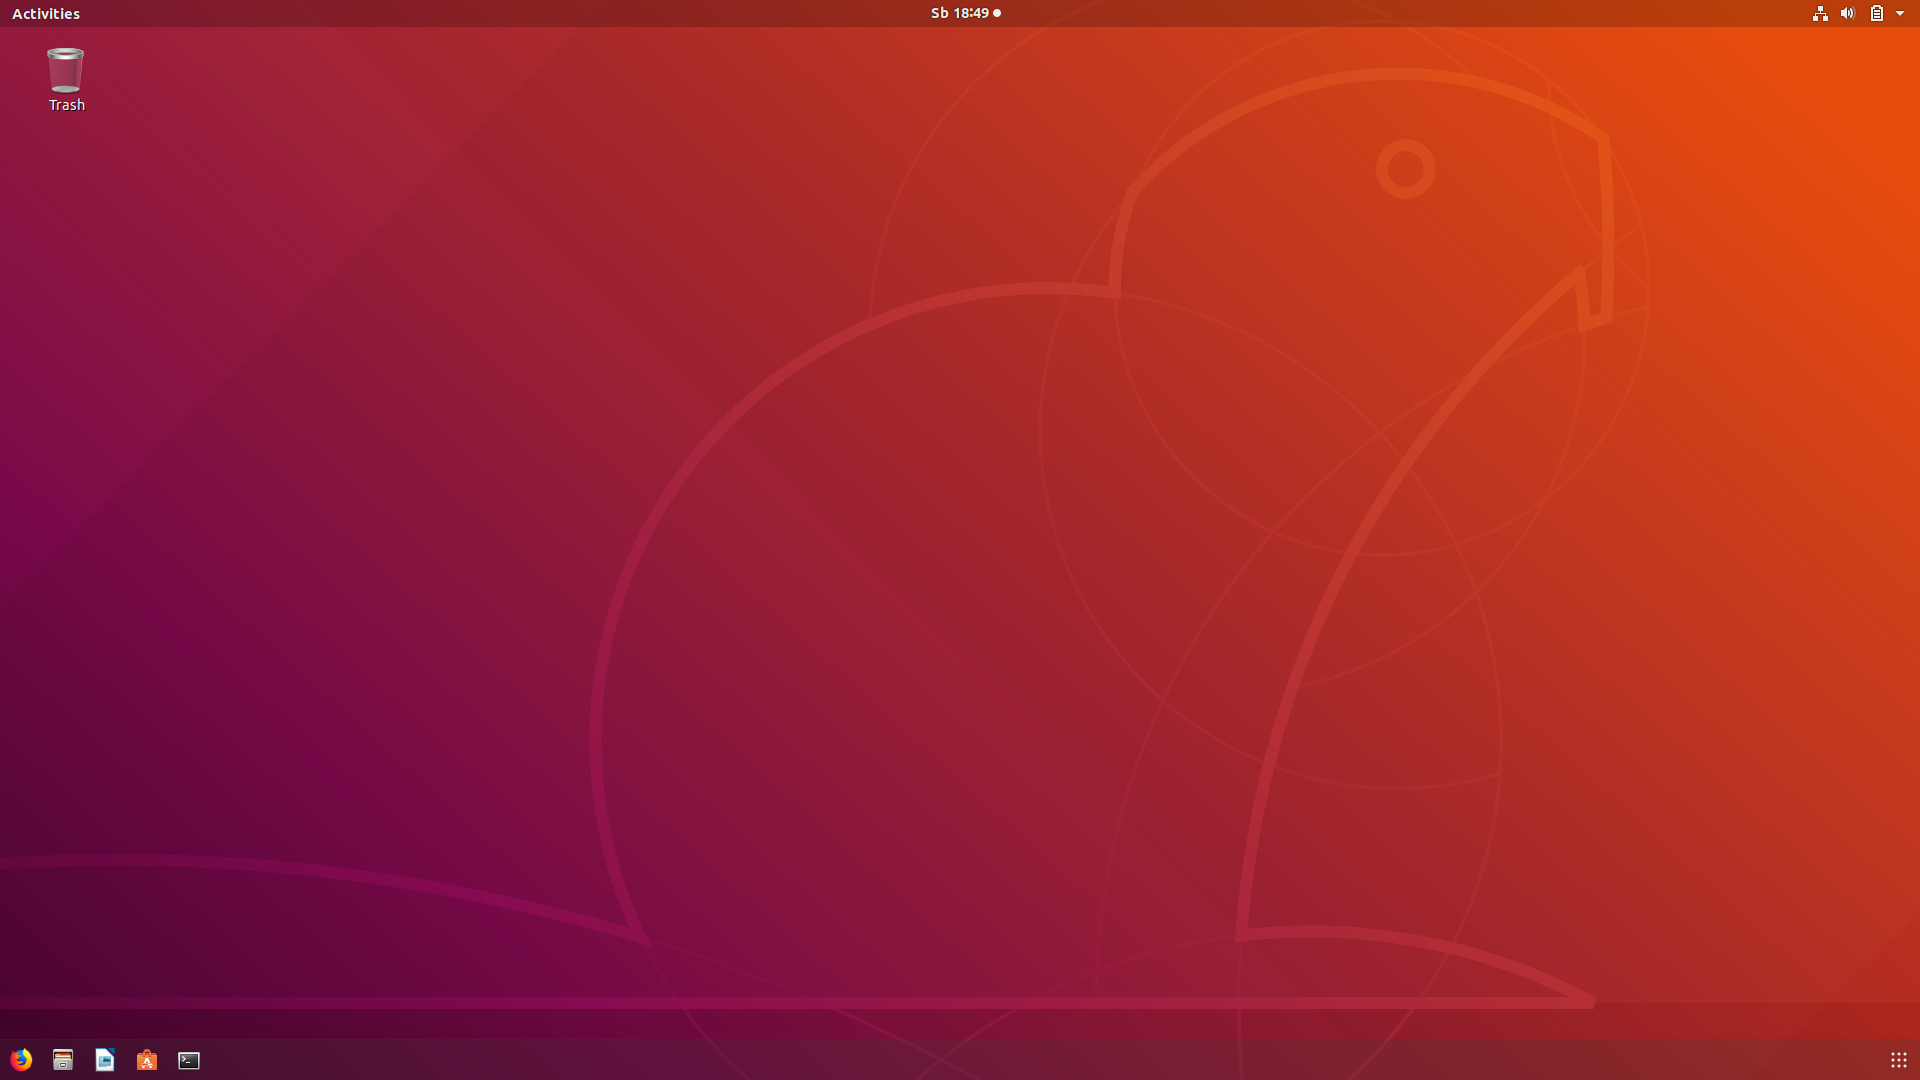
\includegraphics[width=\textwidth]{chapters/00-intro/img/ubuntu.png}
    \caption{Ubuntu}
    \label{fig:intro:distro:ubuntu}
  \end{subfigure}

  \begin{subfigure}[b]{0.6\textwidth}
    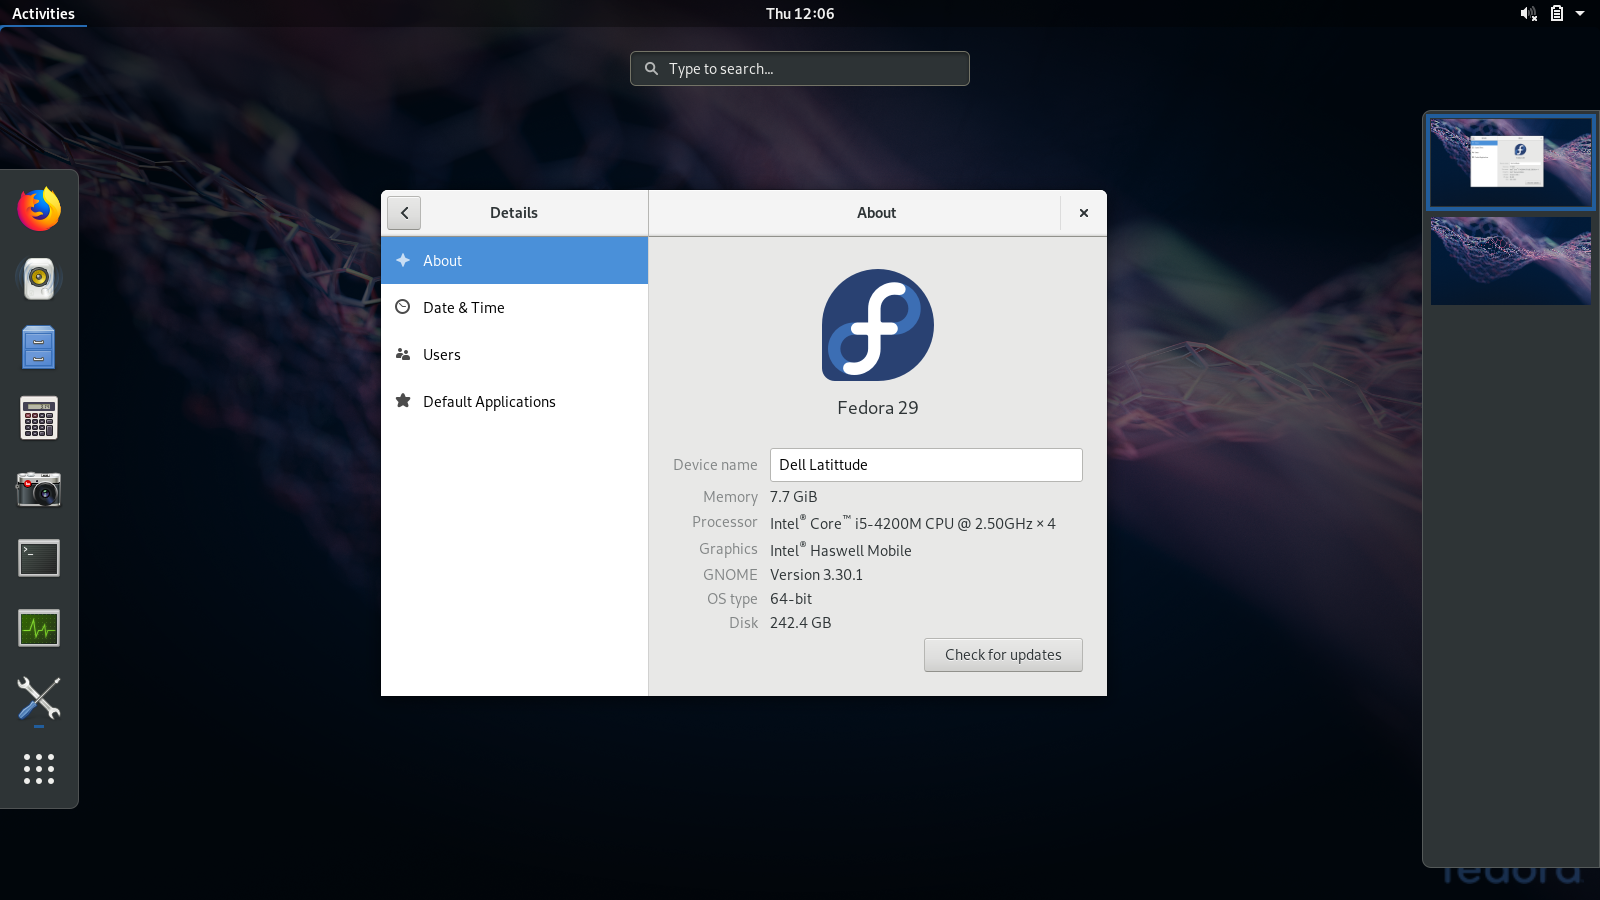
\includegraphics[width=\textwidth]{chapters/00-intro/img/fedora.png}
    \caption{Fedora}
    \label{fig:intro:distro:fedora}
  \end{subfigure}

  \begin{subfigure}[b]{0.6\textwidth}
    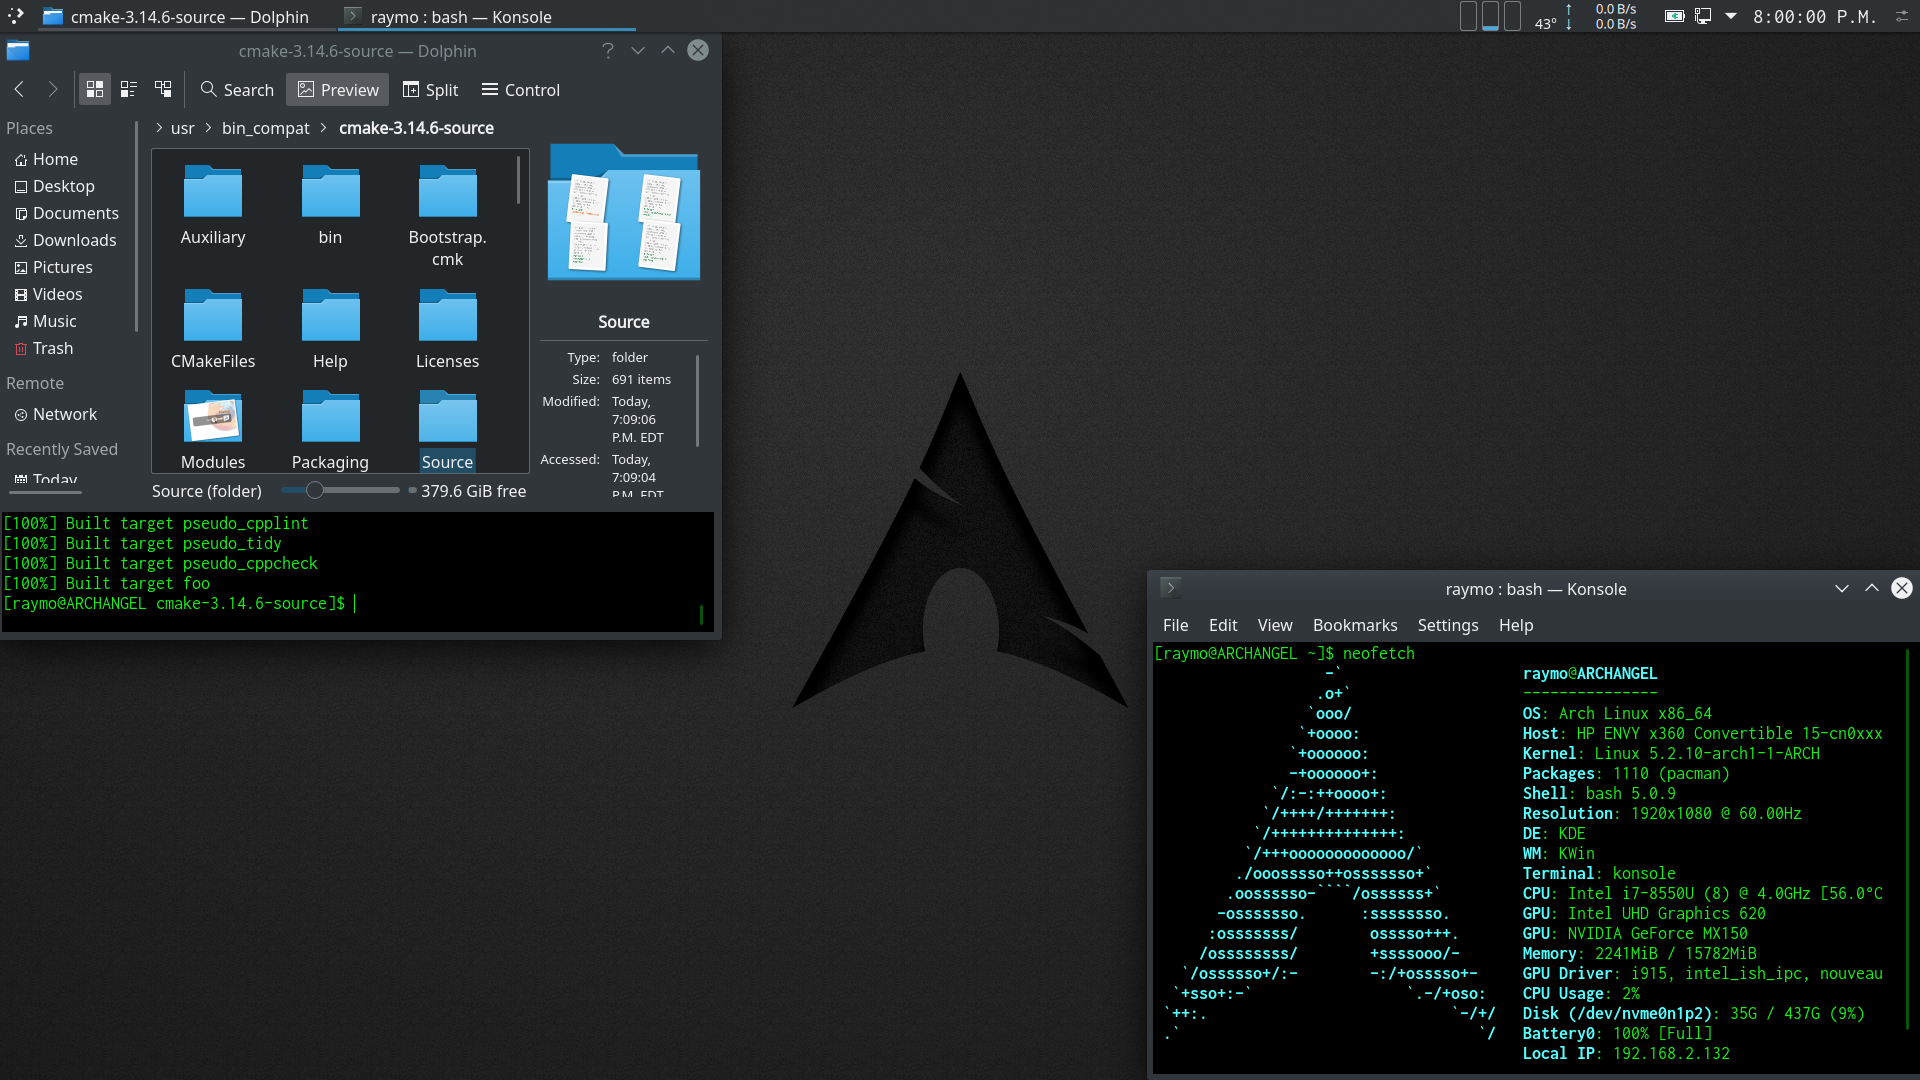
\includegraphics[width=\textwidth]{chapters/00-intro/img/arch.png}
    \caption{Arch}
    \label{fig:intro:distro:arch}
  \end{subfigure}

  \begin{subfigure}[b]{0.6\textwidth}
    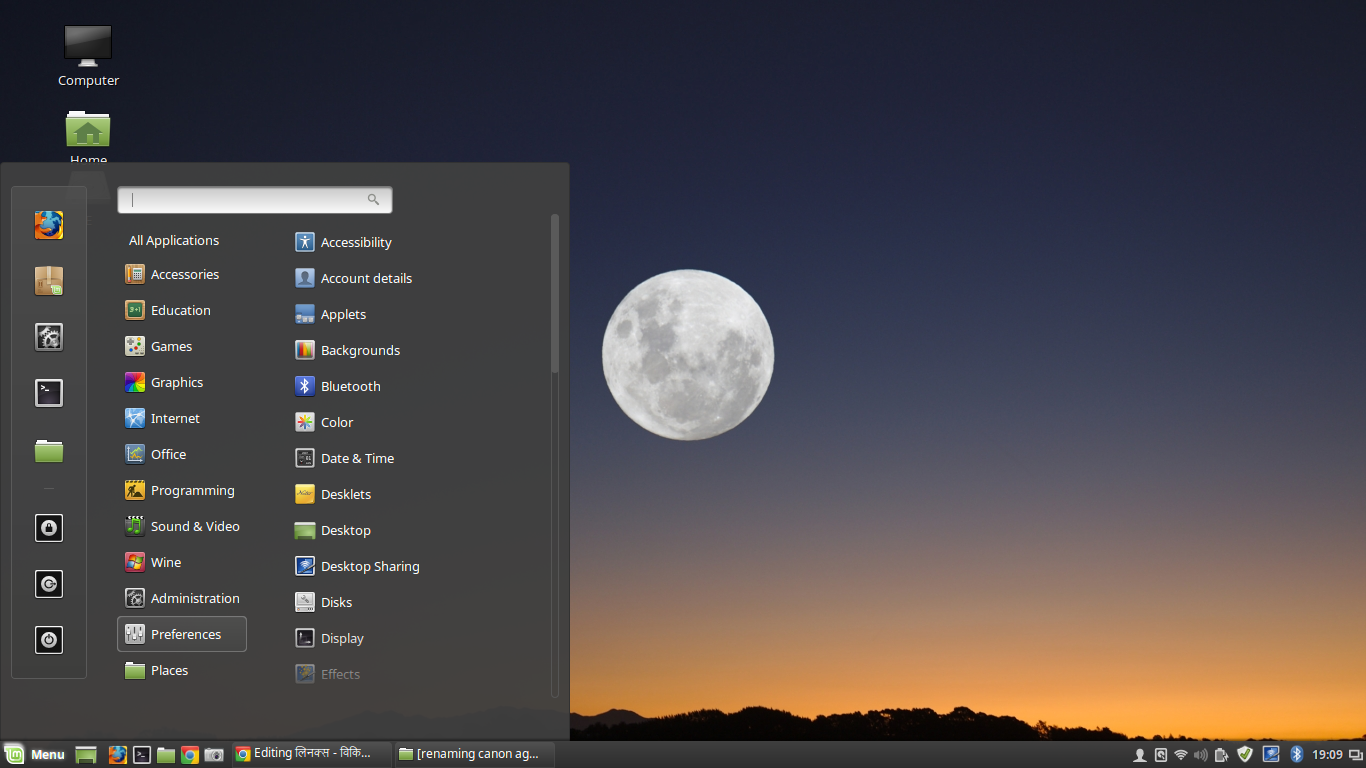
\includegraphics[width=\textwidth]{chapters/00-intro/img/mint.png}
    \caption{Mint}
    \label{fig:intro:distro:mint}
  \end{subfigure}
  \caption{Distribuții Linux}
  \label{fig:intro:distros}
\end{figure}

Fiind una diversă și descentralizată, lumea Linux are multe distribuții. Alegerea unei distribuții ține de factori obiectivi (consum de resurse, hardware pe care rulează, aplicații prezente, personalizare) dar și de unii personali (ce am folosit, ce mi-a plăcut, ce folosesc prietenii mei). Deși interfața poate diferi, elementele software din spate sunt aceleași, așa că un utilizator tehnic nu va avea probleme mari în a se acomoda cu o distribuție nouă.

Distribuțiile Linux pot fi clasificate în familii de distribuții. O familie are la bază o distribuție (care cuprinde anumite aplicații, un mod propriu de gestiune a aplicațiilor, configurări particulare) din care sunt derivate alte distribuții. De exemplu, familia RedHat are la bază distribuția RedHat din care sunt derivate Fedora, CentOS. Familia Debian are la bază distribuția Debian din care sunt derivate Ubuntu și Mint.

Descrieri și comparații între distribuții, argumente pentru a alege una găsiți în număr mare pe Internet și pe site-ul DistroWatch\footnote{\url{https://distrowatch.com/}}. Un sumar al celor mai cunoscute distribuții Linux sunt în \labelindexref{Tabelul}{tab:intro:distro}.

\begin{table}[!htb]
  % TODO: tabel cu cele mai întâlnite distribuții: distribuție, website, sistem de gestiune a pachetelor (referință), interval de lansare
  \caption{Distribuții Linux}
  \begin{center}
    \begin{tabular}{ p{0.13\textwidth} p{0.28\textwidth} p{0.23\textwidth} p{0.25\textwidth} }
      \toprule
        \textbf{Distribuție} &
        \textbf{Site} &
        \textbf{Pachete} &
        \textbf{Interval de lansare} \\
      \midrule
        Debian &
        \url{http://www.debian.org} &
        \texttt{.deb} (\texttt{apt}, \texttt{dpkg}) &
        nefixat \\
        Ubuntu &
        \url{http://www.ubuntu.com} &
        \texttt{.deb} (\texttt{apt}, \texttt{dpkg}) &
        6 luni (aprilie și octombrie) \\
        Fedora &
        \url{https://getfedora.org/} &
        \texttt{.rpm} (\texttt{dnf}, \texttt{rpm}) &
        6 luni (aprilie și octombrie) \\
        Mint &
        \url{http://linuxmint.com} &
        \texttt{.deb} (\texttt{apt}, \texttt{dpkg}) &
        nefixat \\
        Arch &
        \url{http://www.archlinux.org/} &
        \texttt{.deb} (\texttt{pacman}) &
        continuu (\textit{rolling}) \\
        CentOS &
        \url{http://www.centos.org/} &
        \texttt{.rpm} (\texttt{dnf}, \texttt{rpm}) &
        aliniat cu Red Hat Enterprise Linux, nefixat\\
        Kali &
        \url{http://www.debian.org} &
        \texttt{.deb} (\texttt{apt}, \texttt{dpkg}) &
        continuu (rolling) \\
      \bottomrule
    \end{tabular}
    \label{tab:intro:distro}
  \end{center}
\end{table}

\subsection{Mașina virtuală de suport}
\label{sec:intro:vm}

O dată cu această carte oferim o mașină virtuală de suport pe care rulăm părțile aplicative pe care le prezentăm. Mașina virtuală de suport se poate descărca de la adresa TODO și rulează distribuția Ubuntu 18.04. Am optat pentru această distribuție pentru că este printre cele mai cunoscute și pentru că familia Debian cuprinde un număr mare de distribuții (printre care și Ubuntu). Șansele să vă întâlniți cu o distribuție din familia Debian sunt foarte mari.

Mașina virtuală poate fi descărcată și pornită în soluțiile de virtualizare VirtualBox sau VMware. Contul de utilizator este \texttt{student} cu parola \texttt{student}.

\subsection{Instalarea Linux}
\label{sec:intro:linux-install}

Spre deosebire de Windows sau macOS, puține sisteme desktop sau laptop vin cu Linux preinstalat. Așa că majoritatea utilizatorilor vor trebui să instaleze Linux. Așa cum am amintit și mai sus, Linux poate fi instalat direct pe sistemul fizic (singur sau dual-boot cu Windows) sau într-o mașină virtuală. Instalarea pe sistemul fizic are avantajul performanței, pe când cel în mașina virtuală avantajul ușurinței în instalare și a flexibilității.

Nu vom insista pe instalarea Linux. Din nou, resursele din Internet acoperă copios acest subiect. O precizare este că, la fel ca orice alt sistem de operare, este nevoie de un mediu de instalare: un CD-ROM/DVD-ROM bootabil sau, mai probabil, un stick USB bootabil. Astfel, pentru a instala Linux, un utilizator va urma pașii:

\begin{enumerate}
  \item Va descărca un fișier imagine ISO de pe Internet conținând imaginea distribuției Linux care va fi instalată. De exemplu, de la adresa \url{http://releases.ubuntu.com/18.04/} se descarcă fișierul ISO pentru Ubuntu 18.04.
  \item Va crea un mediu bootabil de la fișierul imagine ISO. Va folosi o aplicație de tip ISO image burner ca să scrie imaginea pe CD-ROM/DVD-ROM sau o aplicație precum Unetbootin pentru a scrie imaginea pe un stick USB.
  \item Va porni (boota) sistemul de tip desktop/laptop de pe mediul bootabil creat mai sus.
  \item Va realiza instalarea efectivă. Pașii sunt destul de simpli, majoritatea putând fi realizați prin apăsarea butoanelor de tip \textit{Next} în ecranul de instalare.
\end{enumerate}

\section{Sumar}
\label{sec:intro:summary}

Avem în jur și folosim sisteme informatice compuse din sisteme de calcul interconectate.

Un sistem de calcul este compus din hardware și software. Sisteme de calcul sunt atât laptopuri și dispozitive personale câte și dispozitive de rețea, componente în mașini, smart TV-uri.

Sistemul de operare e componenta software centrală ce asigură accesul utilizatorului (prin aplicațiilor software) la resursele hardware.

În această carte folosim Linux, un sistem de operare open source cu o comunitate largă și care facilitează dobândirea de competențe și cunoștințe tehnice.

Din punct de vedere istoric, Linux este un sistem de operare din familia Unix.

De obicei folosim Linux pe sisteme desktop în forma unei distribuții GNU/Linux ce include sistemul de operare, aplicațiile și interfața. Similar Linux, majoritatea componentelor software sunt open source.

Mașina virtuală de suport a acestei cărți rulează distribuția Ubuntu 18.04.

Linux poate fi instalat lângă Windows în mod dual-boot sau poate fi instalat într-o mașină virtuală, precum cea pusă la dispoziție ca suport al acestei cărți.
